\section{Introduction}

SpaghettiLens is build on top of GLASS and provides a easy to use web based user interface to

1. quickly create models of lenses from any data sources
2. help the comunity to collectivillity work on models
3. help manage, store and evaluate all the data

It was designed to be very modular. It has the potential to run as a stand alone application on ones homecomputer, or as a heavy load web application that can be accessed with mobile phones, tables or regular computers.\footnote{Not all of those use cases are very well tested at the moment}

It was designed to be scalable, so it can be used by many clients in parallel, provided sufficient hardware power. The whole setup can run on a singe machine, or it's components can easily be distributed among many hardware machines. Additional machines\footnote{worker nodes} can be added in a hot plug and play manner. The system needs no restart. The server could even spawn more threads in times on high demand.

It was licensed to be open source (Whatever license, GPLv3??) because only open source software and data formats are the future of mankind.. ;)




\begin{figure}[htbp]
  \centering
    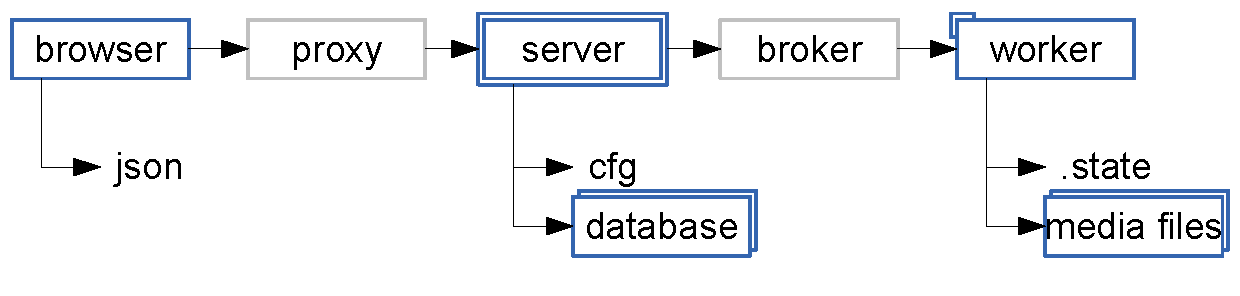
\includegraphics[width=\figwidth]{fig/pipeline.pdf}
  \caption{\spl Setup}
  \label{fig:pipeline2}
\end{figure}